\documentclass[12pt,letterpaper]{article}
\usepackage[top=2cm,bottom=4cm,left=3cm,right=3cm]{geometry}
%PARA IMAGENES
\usepackage{graphicx}
\usepackage{float}
\usepackage{amsmath}
\usepackage{subfig}
%Codificación de Fuente
\usepackage[spanish]{babel}
%\usepackage[english]{babel}
\usepackage[utf8]{inputenc}
\usepackage[T1]{fontenc}
\usepackage{textcomp}
\usepackage{fancyhdr}
\usepackage{enumerate} 
%BIBLIOGRAFIAS
\usepackage{float}
\usepackage[backend=bibtex]{biblatex}
\addbibresource{bibliografia.bib}
%INDICES	
\usepackage{hyperref}
%\makeindex

\begin{document}
\begin{center}
{\Large Universidad Politécnica de Chiapas}\\
{\large Ingeniería en Desarrollo de Software}\\
\vspace{1cm}

\end{center}

\resizebox{15cm}{!} {	
\begin{tabular}{|l|l|}
	\hline 
	\textbf{Cuatrimestre} & \textbf{Agosto- diciembre de 2019} \\ 
	\hline 
	\textbf{Cuatrimestre y grupo} & \textbf{9A} \\ 
	\hline 
	\textbf{Asignatura} & \textbf{Inteligencia Artificial} \\ 
	\hline 
	\textbf{Corte} & \textbf{03} \\ 
	\hline 
	\textbf{Actividad} & \textbf{IA.C3.A2 Entrega final} \\ 
	\hline 
	\textbf{Fecha de asignación} & \textbf{2019.09.23} \\ 
	\hline 
	\textbf{Fecha de entrega Classroom} & \textbf{2019.11.28} \\ 
	\hline 
	\textbf{Fecha de entrega (Revisión)} & \textbf{2019.120.04} \\ 
	\hline 
	\multicolumn{2}{|c|}{} \\ 
	\hline 
	\textbf{Matrícula} & \textbf{Nombre:} \\ 
	\hline 
	171112 & Bartolón Díaz, Alexis de Jesús \\ 
	\hline 
	171122 & Hernandez Jimenez, Milton Neftali\\ 
	\hline 	
\end{tabular} 
}
 
\vspace{3cm}

\begin{center}
{\Huge DESARROLLO DE UNA APLICACIÓN MÓVIL PARA DETERMINAR EL ANÁLISIS DEL SUELO MEDIANTE CROMATOGRAFÍA}
\end{center}



\newpage
\tableofcontents
\newpage
\section{Introduccion}
El proyecto consiste analizar las características de un croma.

\subsection{Objetivo general}
Agilizar el proceso de comparación de resultados de la cromatografía para verificar el estado del suelo. 

\subsection{Objetivos específicos}
\begin{itemize}
\item Análisis de muestra (croma) con una aproximación de diagnostico automático.
\end{itemize}

\section{Marco teórico}
Hoy en día para las personas que practican actividades agropecuarias les es muy
difícil saber qué tan efectivo es sembrar en los terrenos o qué tierras son ricas en
minerales y materia orgánica para las plantas o animales, y por ende pierden
ganado o siembra.
Esto se debe a una falta de conocimiento del cuidado del suelo por parte de las
personas que practican la agricultura o alguna otra actividad agropecuaria , esta
falta de conocimiento puede generar grandes consecuencias en el suelo como por
ejemplo:

\begin{itemize}
\item La pérdida de fertilidad y contaminación que se deben a cambios en la
composición del suelo por el uso de sustancias tóxicas.
\item Erosión, es el desgaste, arrastre y pérdida de partículas de suelo, se produce
por acción del agua y del viento sobre zonas no protegidas.
\end{itemize}

\subsection{Cromatografía del suelo}
\textbf{¿Por qué cromatografía del suelo?}\\
El cromatograma recoge información vital del suelo, donde se puede leer la interacción
de los factores biológicos, químicos y físicos entre estos y con el medio. Esta interacción muestra el grado de calidad que posee el suelo, y si cada uno de los factores está en armonía con los demás, por lo que se sitúa el cromatograma en el centrodonde interactúan los distintos factores.

\begin{figure}[H]
 \centering	
   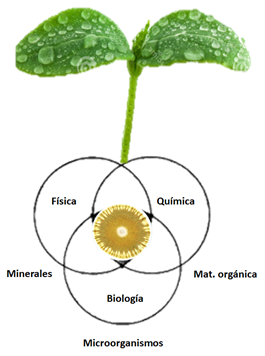
\includegraphics[width=0.4\textwidth]{images/1.png}
   \caption{\textit{Cromatografía interrelaciona la parte física, química y biológica del suelo.}}
   \end{figure}	

En base a estos tres factores mencionados en la Figura 1, la calidad del suelo se compone de tres elementos esenciales para un adecuado funcionamiento (las 3M): los microorganismos, los minerales y la materia orgánica.

\begin{figure}[H]
 \centering	
   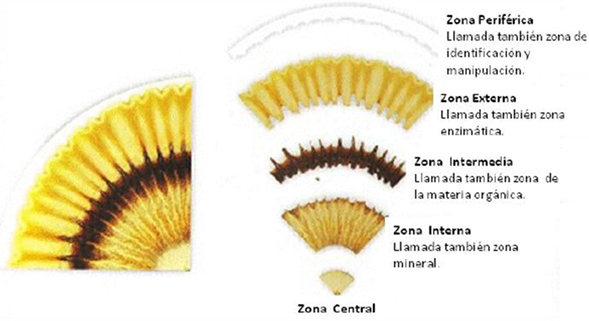
\includegraphics[width=0.7\textwidth]{images/2.png}
   \caption{\textit{Zonas de una cromatograma.}}
   \end{figure}	
\newpage
\section{Desarrollo del proyecto}

Para  llevar  a  cabo  el  diseño  y  desarrollo  de  este  proyecto  se  consultaron numerosas  paginas web sobre procesamiento de imágenes y  se  realizaron continuas reuniones con el tutor sobre las dudas que surgían mediante el desarrollo del proyecto.

El principal objetivo de este proyecto es:

\begin{itemize}
\item Hacer uso de un sensor.
\item Recuperar características a través de procesamiento de señales.
\item Utilizar una red neuronal de retropropagación con validación cruzada.
\item Realización de un conjunto de  algoritmos  que  realicen  las  funciones  de  detección  y  reconocimiento  de  patrones de forma eficiente.
\end{itemize}

\subsection{Equipo utilizado}
A continuación se describirá todo  el  material  requerido  para  el  desarrollo  del proyecto, con la finalidad de esclarecer el porqué de la elección de éstos.Se
describirá tanto  el  equipo requerido,  necesario  para  la  instalación  de  programas  y la  simulación de nuestra aplicación, como el software utilizado durante la programación de ésta
\subsubsection{Hardware}
Se han utilizado, dos ordenadores, que cuentan las siguientes especificaciones:
\begin{itemize}
\item Sistema operativo Linux.
\item Procesador Intel Celeron N3060 @ 2x 2.48GHz
\item Memoria Ram de 4GB.
\item 500 GB de memoria de disco duro.
\item Una resolución de pantalla de 1280 x 800.
\end{itemize}

Para la emulación e instalación de nuestra aplicación, también se ha hecho uso de un Smartphone con un sistema operativo Android y cámara incorporada. En este caso se ha utilizado un Smartphone Huawei P10 con la versión de Android 8.

\subsubsection{Software}
\begin{itemize}
\item Android-Studio
\item Libreria OpenCV.
\item Libreria Sclearn
\item Micro framework Flask
\end{itemize}

\subsection{Características de la Aplicación}
El trabajo desarrollado cuenta con las siguientes características:
\begin{itemize}
\item Captura fotografía de un croma y se sube aun servidor.
\item La red neuronal detecta y reconoce si el croma es valido o no.
\item Contiene una interfaz gráfica para facilitar el uso de la aplicación.
\end{itemize}

Todo el procesamiento de imágenes y la red neuronal se ha implementado en python3.


\subsection{Patrones a detectar}

Un croma contiene varias características que determinan si la calidad del suelo se encuentra en buenas condiciones. 

\begin{figure}[H]
 \centering	
   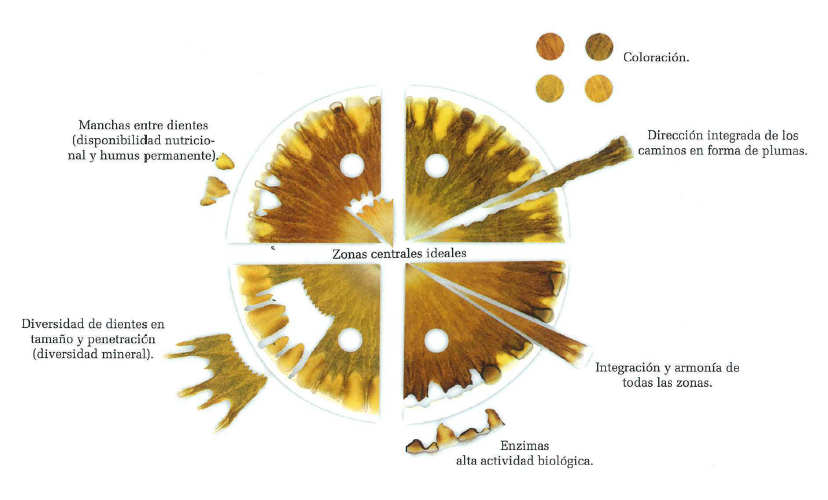
\includegraphics[width=0.8\textwidth]{images/3.png}
   \caption{\textit{Características de un croma.}}
   \end{figure}	
   
Tal y como se observa en la Figura 3, existe una variedad de características que contiene un croma.
El número  de  características a detectar en el programa son ocho que son importantes para saber la calidad del estado del suelo.
Estas características son: 
\begin{itemize}
\item Contorno.
\item Lineas.
\item Colores como el negro, gris, violeta, verde y azul.
\item Dientes de caballo.
\item Patrón de figura (Dientes de caballo)
\end{itemize}


\subsection{Extracción de características}


La extracción de las 8 características anteriormente mencionadas son los datos de entrada que la red neuronal necesita para detectar si el croma es valido o no.

A continuación se presentan más en detalle como se realizo la extracción de características mediante procesamiento de imagen.

\subsubsection{Detección de contorno}

\subsubsection{Detección de lineas}
\subsubsection{Detección de colores}
\subsubsection{Detección de patrones}



\subsection{Validación cruzada}



\subsection{Red neuronal de retropropagación}
Scikit-learn (anteriormente scikits.learn) es una biblioteca para aprendizaje de máquina de software libre para el lenguaje de programación Python.

Con Scikit-learn fue implementada la red neuronal, dado a que es una de las mejores librerias de python y con facil aprendisaje, segun la comunidad de desarroladores en AI en el lenguaje de python.

Se hizo uso de la libreria de pandas para que el dataset este cargado en el sistema desarrollado, esta libreria nos permitio tener un mejor manejo de la información, que se necesitaba para recuperar los datos necesarios en la elavoracion de la validacion cruzada, el entreno y el testeo. 

Por ultimo, scikit-learn tiene una de las funciones que permite guardar el mejor modelo obtenido y hacer uso de esta para las pruebas del sistema.

https://iartificial.net/librerias-de-python-para-machine-learning/#scikit-learn



\section{Resultados obtenidos}

 
\addcontentsline{toc}{section}{References}
\printbibliography

\end{document}
